%#####################################################
\section{Datasets}
\label{sec:data}
%#####################################################

This section describes the datasets and catalogs used in this analysis. 

%\todo{rephrase those sub-sections so they are not a copy/paste of the other paper and tweak them for relevance with regards to the focus of this paper}
%\tianqing{I took the liberty to re-word this section and added a bit of text}

%\todo{can we reuse figures 1 and 2 as is ? what tweaks do we want to make ?}

%#####################################################
\subsection{HSC-SSP PDR3 Shape Catalog}
\label{sec:data:hsc}
%#####################################################

The Hyper Suprime-Cam Subaru Strategic Program (HSC-SSP) is a wide and deep imaging survey conducted by the 8.2-meter Subaru Telescope. The weak lensing shear catalog used in this study is the HSC S19A galaxy shape catalog, i.e., the so-called HSC Year 3 shear catalog\cite{HSCShapeCataloguePDR3Li2022}, an intermediate release between the HSC Public Data Release 2 (PDR2) \cite{hsc_pdr2} and HSC Public Data Release 3 (PDR3) \cite{HSC2022datarelease3}. This catalog builds upon $i_{\mathrm{band}}$ imaging data obtained from 2014 to 2019 in the Wide fields of the HSC survey, at a mean $i_{\mathrm{band}}$ PSF Full-Width of Half-Maximum (FWHM) of $0.59''$ \cite{HSCShapeCataloguePDR3Li2022}. A conservative $i_{\mathrm{band}}<24.5$ magnitude cut is applied to the dataset. Even with the conservative magnitude cut, the catalog has an effective number density of $19.9 {\;\rm arcmin}^{-2}$. The geometric footprint of the catalog is split into 6 fields: \texttt{HECTOMAP}, \texttt{XMM}, \texttt{VVDS}, \texttt{GAMA09H}, \texttt{GAMA15H} and \texttt{WIDE12H}.

%In the first tomographic bin calibration study, 
We adopt consistent tomographic binning to the HSC Y3 cosmic shear \cite{Li2023_HSCY3_CosmicShear, Dalal2023CosmoShearHSC} and tomographic $2\times2$pt\cite{Zhang2025aTomographic2x2pt} and $3\times2$pt analysis\cite{Zhang2025bTomographic3x2pt}, which uses $z_{\rm best}$ (defined in \cite{HSCPHotozTanaka2017}) of \texttt{DNNz} to assign galaxies into four tomographic bins, using $z=0.3, 0.6, 0.9, 1.2,1.5$ as bin edges. 
In addition, a \textit{quality control cut} is applied to the first and second tomographic bins, which depends on the $95\%$ confidence interval boundaries of the \texttt{DNNz} \cite{DNNZHSCNishizawa2020} and \texttt{Mizuki} \cite{MizukiHSCTanaka2015} photometric redshift algorithms,
\begin{equation}\label{eq:calib_cut}
(z^{\texttt{DNNz}}_{95,\,\mathrm{max}}-z^{\texttt{DNNz}}_{95,\,\mathrm{min}})<2.7\;\;\&\;\;(z^{\texttt{Mizuki}}_{95,\,\mathrm{max}}-z^{\texttt{Mizuki}}_{95,\,\mathrm{min}})<2.7.
\end{equation}
This selection is performed in order to remove possible double-peak galaxies with photo-$z$ probability density functions reporting multi-modal distributions with a second, smaller peak around $z\sim3$. The cut removes $\sim31\%$ of sources in the first bin, and $\sim8\%$ of sources in the second bin \cite{HSCClusteringRau2023}.


In the rest of this analysis, when using redshifts outside of the HSC tomographic bins, the quality control cut is applied to all sources with redshifts between $z\sim0$ and $z\sim0.3$, which removes about $\sim16\%$ of the sources within that redshift range. The fiducial redshift value kept to determine if a redshift is included in a bin or not is $z_{\mathrm{best}}^{\texttt{DNNz}}$. The $_\mathrm{best}$ subscript notes the redshift point estimate that minimizes the risk function, $R(z_{\mathrm{p}})=\int P(z)L(\frac{z_{\mathrm{p}}-z}{1+z})\mathrm{d}z$, based on the individual probability density function $P(z)$ obtained through $\texttt{DNNz}$, and with $L(x)$ a loss function. More details can be found in the following works \cite{HSCPHotozTanaka2017, DNNZHSCNishizawa2020}.

%#####################################################
\subsection{The DESI-Calibrated HSC Y3 $n(z)$}
\label{sec:data:desi}
%#####################################################

This work presents updated cosmic shear constraints using the calibrated HSC Y3 $n(z)$ distributions obtained in the companion paper \cite{ChoppinDeJanvry2025a}. In that work, we use DESI Data Release 1 (DR1) and DR2 to recover the redshift distribution of the four aforementioned tomographic bins by leveraging the spatial clustering of galaxies via the clustering redshifts method. 
The Dark Energy Spectroscopic Instrument is an eight year multiplexed spectroscopic program started in 2021, conducting a survey of $17,000$ deg$^2$ of the sky, covering spectroscopic redshift ranges up to $z\sim4.2$. As such, it provides an unprecedented reference spectroscopic dataset to calibrate photometric redshifts. 
We measure the angular cross-correlation between the HSC Y3 photometric sample and the DESI spectroscopic reference samples as a function of the spectroscopic redshift. Since galaxies at similar redshifts are physically clustered together, the cross-correlation signal peaks when the photometric and spectroscopic samples overlap in true redshift space, even if the photometric redshift estimates are biased or uncertain. 

\begin{figure}[ht]
    \centering
    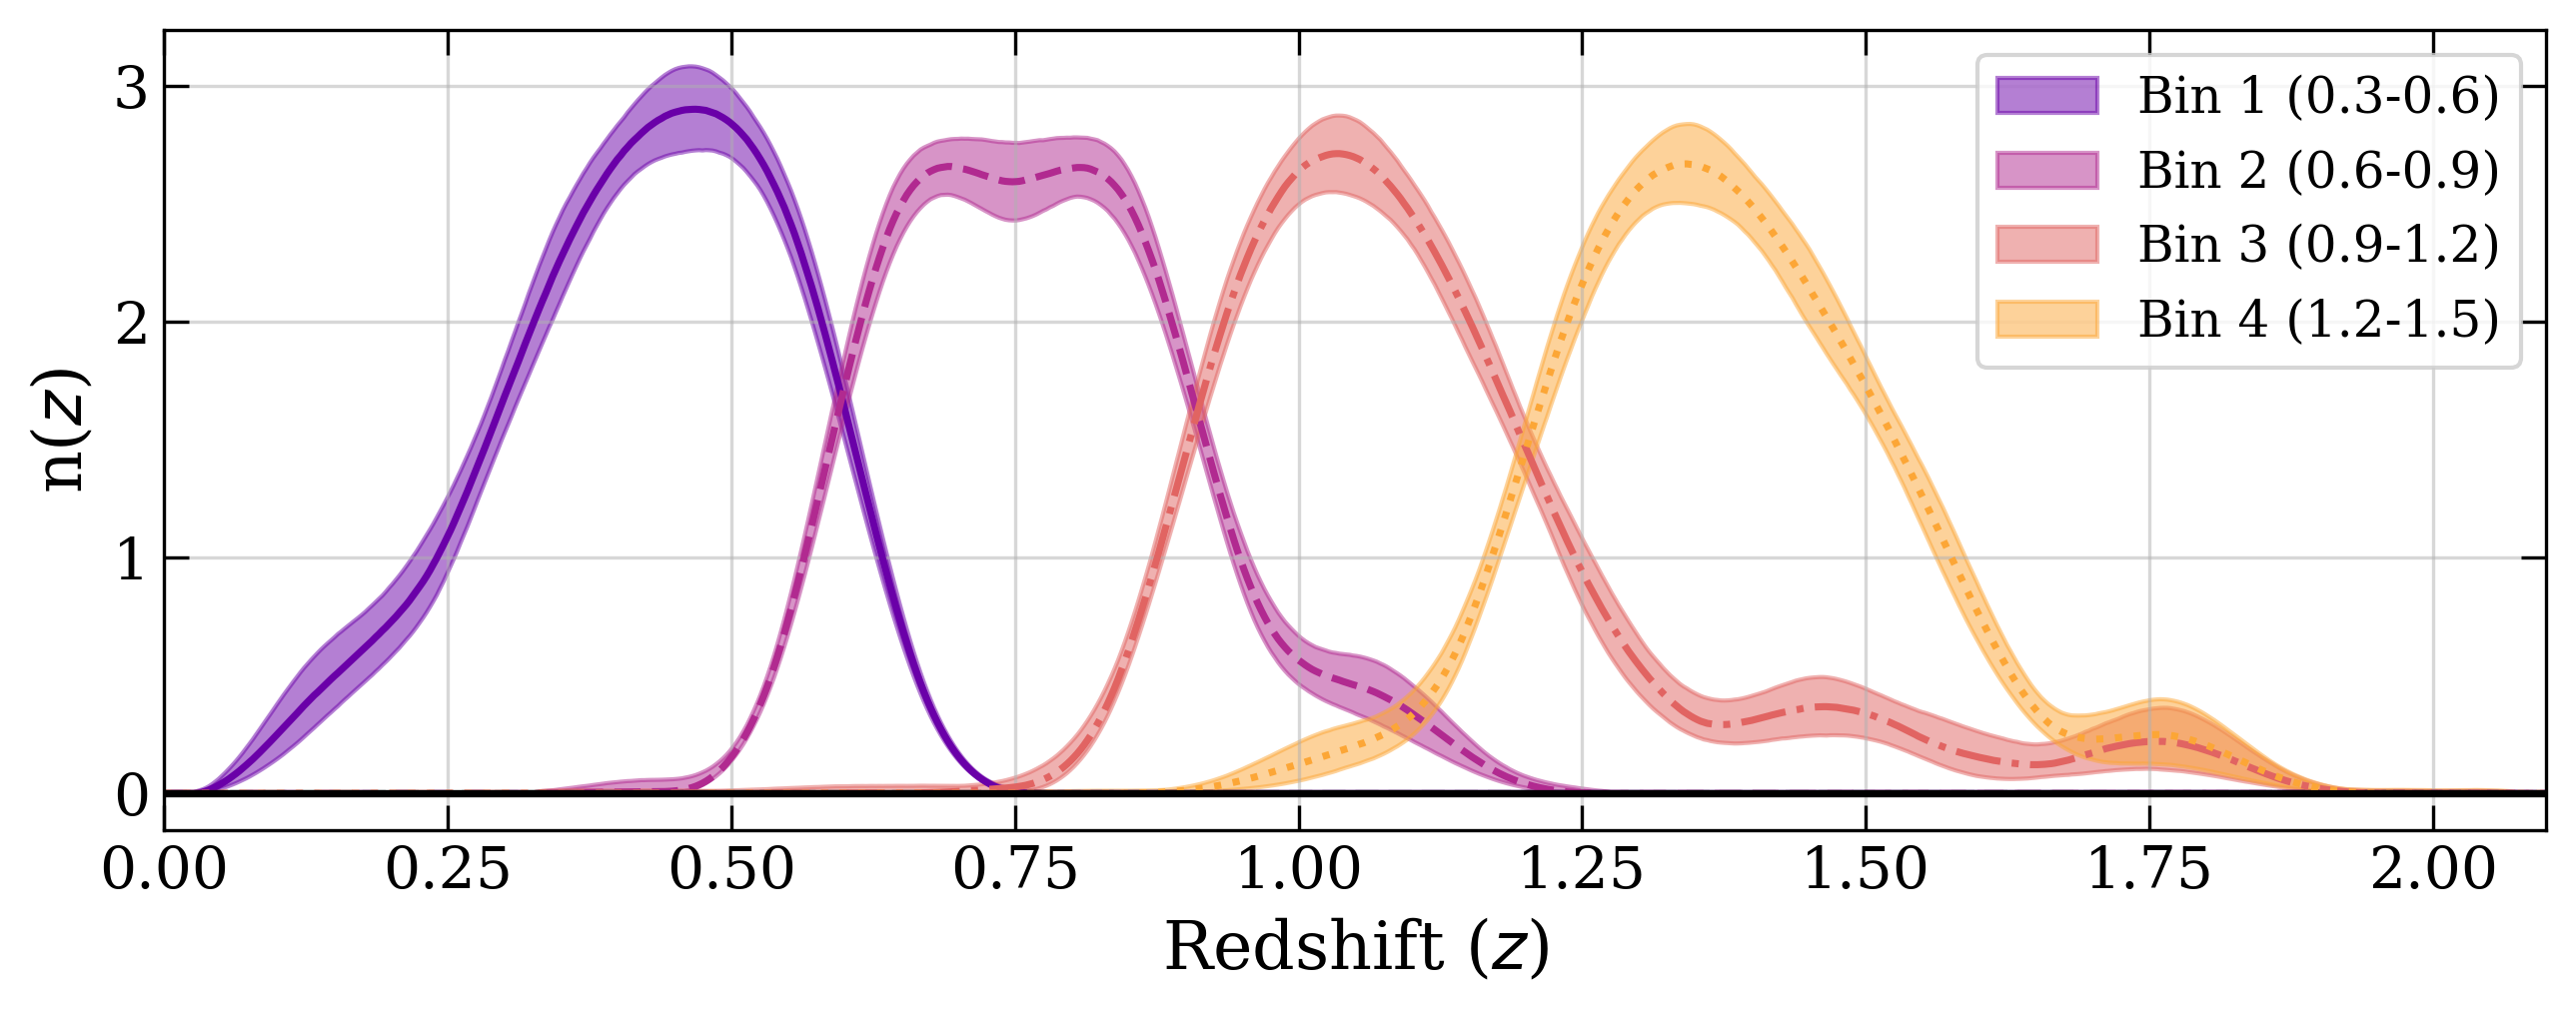
\includegraphics[width=0.95\textwidth]{img/all_tomo_cshear.png}
    \caption{$n(z)$ distributions for each of the 4 tomographic Bins, spanning $z_p\sim0.3$ to $z_p\sim1.5$ where $z_p$ is the best estimate of the \texttt{DNNz} photo-$z$ algorithm \cite{DNNZHSCNishizawa2020} used for tomographic Bin selection, as described in section \ref{sec:data:hsc}. The $n(z)$ for each Bin is displayed with the median posterior sample and the $1\sigma$ widths adapted from \cite{ChoppinDeJanvry2025a}. Here, the $n(z)$ shown includes all corrections to galaxy bias and magnification effects.}
    \label{fig:all_tomo}
\end{figure}

We analyze how the cross-correlation amplitude varies with spectroscopic redshift, characterize and model systematic biases (including galaxy bias from both the spectroscopic and photometric samples and magnification effects) and finally, we reconstruct a fully DESI-calibrated underlying redshift distribution $n(z)$ of the four tomographic bins of the HSC Y3 photometric sample, displayed in figure \ref{fig:all_tomo}. In the clustering redshifts analysis, we include two scale cuts used for two-point correlation functions in the $n(z)$ calibration measurement ($0.3-3$h$^{-1}$Mpc and $1-5$h$^{-1}$Mpc). The smaller scale cut remains the fiducial measurement of this work: however, we make use of both scale cuts for consistency purposes, as presented in section \ref{sec:results}. For more details on the methodology followed, we refer the reader to Choppin De Janvry {\it et al.} (2025a) \cite{ChoppinDeJanvry2025a}. 

%Compliance with DESI internal policies required the use of DESI DR2 to be limited to the calibration of the two highest HSC tomographic bins: $0.9 < z_{\mathrm{p}}\leq1.2$ and $1.2 < z_{\mathrm{p}}\leq1.5$. We use the public DESI DR1 dataset for the remaining tomographic bins: $0.3 < z_{\mathrm{p}}\leq0.6$ and $0.6 < z_{\mathrm{p}}\leq0.9$. 
%For measurements on tomographic bins different from the fiducial HSC \cite{HSCClusteringRau2023, CosmoShearLi2023HSCY3, Dalal2023CosmoShearHSC} ones (e.g. section \ref{sec:modeling:photoz_gal_bias}), DR1 is used for any tomographic bin such that $z_{\mathrm{p}}\lesssim0.9$, and DR2 elsewhere ($z_{\mathrm{p}}>0.9$), where $z_{\mathrm{p}}$ is the center of the tomographic bin. 
%The DESI dataset is further described hereafter, in section \ref{sec:data:desi}. 
%The photometric sample we calibrate is the S19A HSC-SSP PDR3 Shape Catalog (HSC) \cite{HSCShapeCataloguePDR3Li2022}, described in \ref{sec:data:hsc}. Each of the three catalogs is displayed in Figure \ref{fig:footprint}.


%\begin{figure}[h]
%    \centering
%    
\includegraphics[width=0.95\textwidth]{img/sec2/footprint.png}
%    \caption{Sky coverage of DESI DR1 (navy outline), DR2 (in background density map, including all target classes in the number of galaxies $\mathrm{N}_g$) and HSC Year 3 (red outline), with the galactic plane (gray line). The HSC data lands in areas of high overall completeness for DESI, as these areas were targeted in priority. DESI DR2 improves over DR1 with better overall completeness, especially for the ELGs and in the northern \texttt{HECTOMAP} field (roughly $\mathrm{RA}\sim40^\circ$, $\mathrm{DEC}\sim240^\circ$).}
%    \label{fig:footprint}
%\end{figure}

%For both DESI DR1 and DR2, calibrations are performed with the Large Scale Structure (LSS) catalogs of the DESI survey \cite{DESIConstructionLSS2024}. The LSS catalogs provide weighted clustering and random catalogs tailored to the specifics of the DESI survey for each of the target classes %(and sub targets) 
%used. The LSS catalogs take into account imaging systematics, selection and footprint effects, possible redshift failures, tiling overlap, as well as other effects -- the full description of which can be found in the DESI data model\footnote{\href{https://desidatamodel.readthedocs.io/en/latest/DESI_ROOT/survey/catalogs/RELEASE/LSS/SPECPROD/LSScats/VERSION/data_clustering.html}{\textcolor{blue}{https://desidatamodel.readthedocs.io/}}} and in in refs \citep{DESIConstructionLSS2024, DESI.2024.II.SampleDef}. 

%This work uses multiple target classes: the BGS  \cite{DESI.Selection.BGS.Hahn2023}, the LRGs \cite{DESI.Selection.LRG.Zhou2023}, the ELGs \cite{DESI.Selection.ELG.Raichoor2023} and the QSOs \cite{DESI.Selection.QSO.Chaussidon2023} as described above. 
%The target classes redshift ranges used in this study are described in Table \ref{tab:desi_z_bounds}, per data release, and the redshift density distribution for both data releases over the HSC footprint is showcased in Figure \ref{fig:density_z}. 
%DESI uses priority ranking to perform fiber assignment on targets \cite{FiberSystem.Poppett.2024}. 
%For the ELG sample, our analysis uses the LOw-Priority (LOP) sample \cite{DESI.Selection.ELG.Raichoor2023} when calibrating with DR1, which has a selection of higher priority ELGs at $1.1\lesssim z\lesssim1.6$. 
%For DR2, in addition to LOP, we use the Very LOw priority (VLO) sample for ELGs, which focuses on targets in $0.6\lesssim z\lesssim1.1$. Indeed, the addition of VLO to the LSS catalogs is a new feature of DR2 compared to DR1.

%\begin{table}[h]
%\centering
%\caption{Redshift ranges as inclusive bin edges used for each data release per tracer.}
%\begin{tabular}{c|c|c}
%\hline
%\textbf{Tracer} & \textbf{DR1} & \textbf{DR2} \\
%\hline
%BGS & $0-0.5$ & $0-0.6$ \\
%LRG & $0.4-1.1$ & $0.3-1.2$ \\
%ELG (LOP) & $0.8-1.6$ & - \\
%ELG (LOP+VLO) & - & $0.7-1.6$ \\
%QSO & $0.8-2.8$ & $0.7-2.8$ \\
%\end{tabular}
%\label{tab:desi_z_bounds}
%\end{table}

%Note that for DR2, some sources are expected outside of the bounds described in Table \ref{tab:desi_z_bounds} and shown in Figure \ref{fig:density_z}.
%Their lower number densities and negligible overlap with the two highest redshift tomographic bins of HSC motivates our choice for redshift cuts. 
%For example, information from low redshift ELGs ($\lesssim0.7$) is not included.


%\begin{figure}[ht]
%    \centering
%    
\includegraphics[width=0.95\textwidth]{img/sec2/density_z.png}
%    \caption{\textit{Upper panel:} N(z) angular density per redshift from the HSC catalog, using photometric redshifts from the \texttt{DNNz} algorithm \cite{DNNZHSCNishizawa2020}. The effect of the calibration cut on HSC is displayed, removing problematic sources up to $z_{\mathrm{best}}^{\mathtt{DNNz}}\leq0.9$ (dotted histogram), as well as HSC's four tomographic bins (shaded colors, including the calibration cut). \textit{Lower panel:} N(z) angular density per redshift of the DESI Large Scale Structure clustering catalogs \cite{DESIConstructionLSS2024}, showcasing the combined tracers distribution (light blue) in the HSC footprint and individual tracers (BGS, ELG, LRG and QSOs). DR1 is represented in dotted lines and DR2 is represented in full lines. In this figure, ELGs are distinguished between ELG-LOP (DR1 analysis) and ELG-LOP+VLO (DR2 analysis). Since most of the HSC footprint is already included in DR1, adding DR2 does not provide an improvement as big as one could expect (cf.  Figure \ref{fig:footprint}). Per tomographic bins, the effective number density counts are 3.77, 5.07, 4.00 and 2.12 arcmin$^{-2}$ \cite{PSFModellingHSCZhang2023} after applying the calibration cut.}
%    \label{fig:density_z}
%\end{figure}
